\chapter{Method}


\begin{figure}[h]
 \begin{center}
  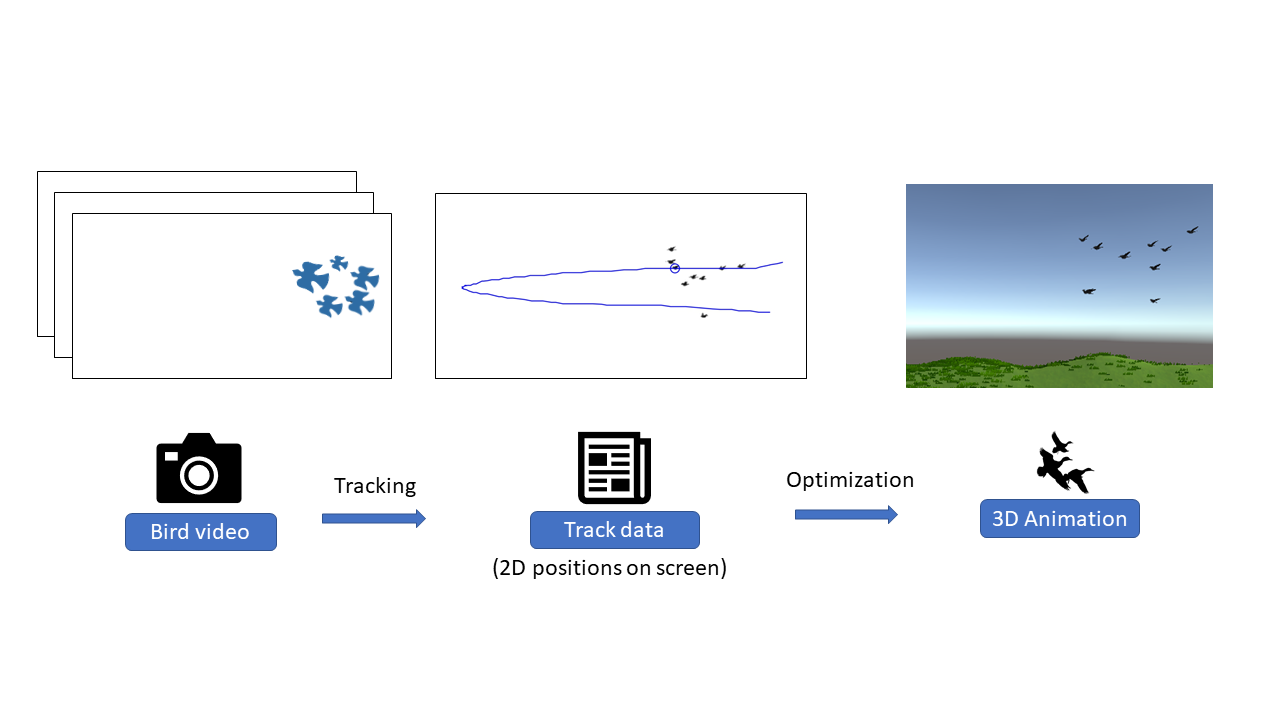
\includegraphics[width=1.0\textwidth]{system.eps}
 \end{center}
 \caption{Method overview}
 \label{figure:system}
\end{figure}


\section{Method overview}


\begin{figure}[h]
 \begin{center}
  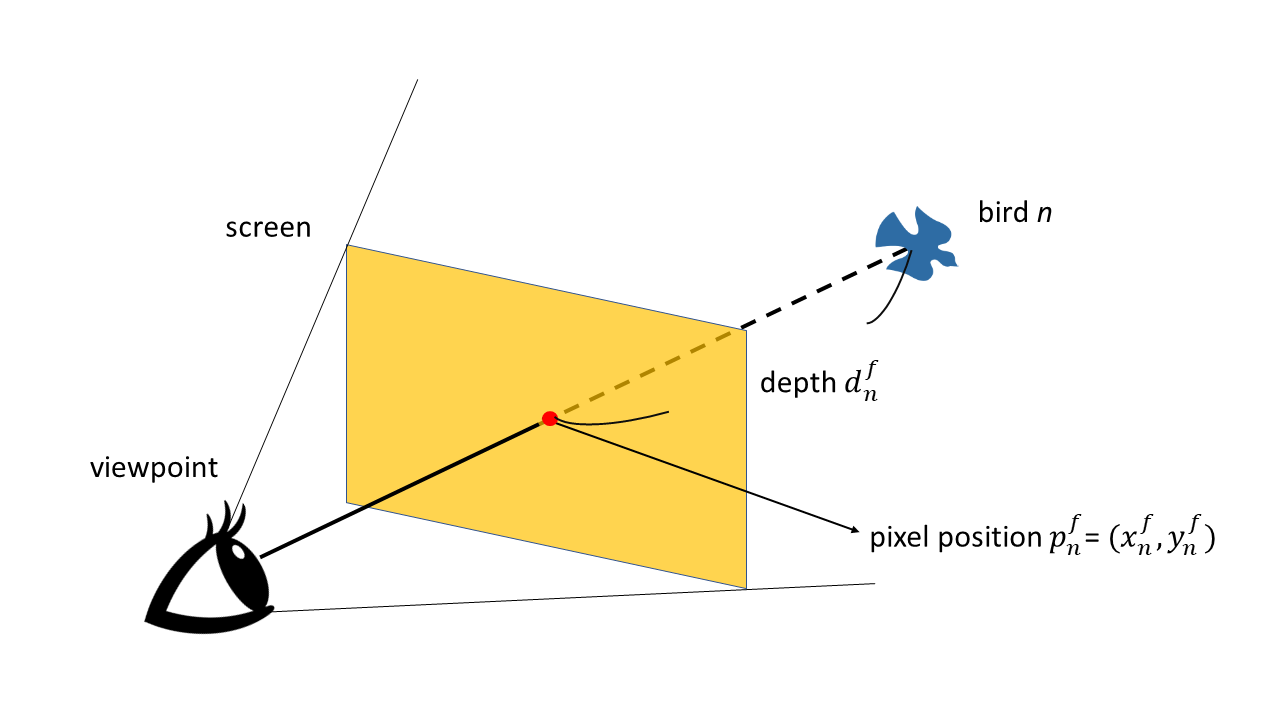
\includegraphics[width=1.0\textwidth]{view.eps}
 \end{center}
 \caption{View scenario in frame $f$.}
 \label{figure:view}
\end{figure}


Figure \ref{figure:system}  shows an overview of our method. As mentioned in Chapter 1, our method synthesizes three-dimensional bird flock motion from input video by predicting depths for each bird in each frame. First, trace data of each bird in the video is retrieved from input video. With the interactive feature tracking technique, track data, which contains two-dimensional projection position trajectory of each bird, can be retrieved with the help of user's indications. Next, depth for each bird in every frame is predicted in optimization step. The goal of predicting depth is to maintain the quality of flight trajectory, which is separated in two terms: trajectory smoothness and flock behavior similarity. These two terms will be discussed in later sections. Here, we consider an image sequence of length $F$ frames as input, with $N$ birds in each frame. Track data contains two-dimensional projection of each bird in the input video. The set of track data is denoted $P=\big\{p_n^f\big\}_{n=1...N,f=1...F}$ , where $p_n^f=(x_n^f, y_n^f)$, representing two-dimensional projection on screen, as shown in Figure \ref{figure:view}. We want to predict depth $d_n^f$ of bird $n$ in frame $f$, while maintain the two properties above. The quality of a flight with a candidate depth set $X=\big\{d_n^f\big\}_{n=1...N,f=1...F}$ can be defined as:


\begin{equation}\label{eq:1}
 E(X) = \sum_{n = 1}^{N} \sum_{f = 1}^{F}e(n,f)
\end{equation}


\begin{equation}\label{eq:2}
 e(n,f) = \lambda_tt(p_n^f, p_n^{f-1},d_n^f) + \lambda_ff(p_n^f, p_n^{f-1},d_n^f)
\end{equation}


$e(n,f)$ denotes error function for bird n in frame f, which includes a trajectory smoothness term $t(.)$, and a flock behavior term $f(.)$. $\lambda_s$ and $\lambda_t$ are tuning parameters corresponding to trajectory smoothness and flock behavior. Thus, the predicting problem can be restated as an optimization problem: choose $X$ to minimize $E(X)$. After the optimal $X$ is found, with the predefined camera parameter and optimal depth $d$, we can get world position of the bird from its screen position.


In most simulation system, velocity of an object is calculated upon mass and force in simulation steps. However, since our optimization method is over frames, we use position-based dynamics system \cite{PBD}, in which velocity in frame f is denoted as

\begin{equation}\label{eq:3}
 \vec{v(f)} = b(f)-b(f-1)
\end{equation}

where $v(f)$ denotes velocity, and $b(f)$ denotes bird position in world space. This makes our optimization system simpler and faster: we can calculate velocity of each bird in current frame and do not need to keep track of it. Although position-based dynamics system is not physically accurate, since our goal is to make visually plausible flock motion, we use it in our system.
For $s$ and $t$ in equation \ref{eq:2}, we use the simple Euclidean distance function on the two positions. We have also experimented with an acceleration term, of the form $s(p_n^f, p_n^{f-1}, p_n^{f-2})$, but it increases the computation cost, and do not produce better result. Details of each term will be discussed in the following sections.


\section{Bird tracking}


To obtain trajectory of each bird in the input video, tracking technique is used in our method. We use an existing tracking system ZooTracer\cite{ZooTracer}, developed by Microsoft research, to do the task. ZooTracer is based on interactive feature tracking technique, proposed by Buchanan and Fitzgibbon \cite{Tracking}. With the tracking system, after preprocessing is done, the user can make tracking data interactively from input video in real time. The system predicts the trajectory of single bird in the video based on user's initial indication. If the tracking is wrong in some frames, user can provide keyframe features by few clicks and improve the track.
The main challenge of using interactive feature tracking on tracking birds is distinguishing between tracked birds. The system records fixed-size image patches for tracking feature points, such as eye on a face. However, in case of tracking bird flock, all birds look similar in small patches. It leads to many errors found in the result, making wrong tracking data. Therefore, more manual manipulations need to be done to get an optimal track. On average, user can complete the track data of one bird in a 200-frame video in less than 1 minute.



\section{Trajectory smoothness}


\begin{figure}[h]
 \begin{center}
  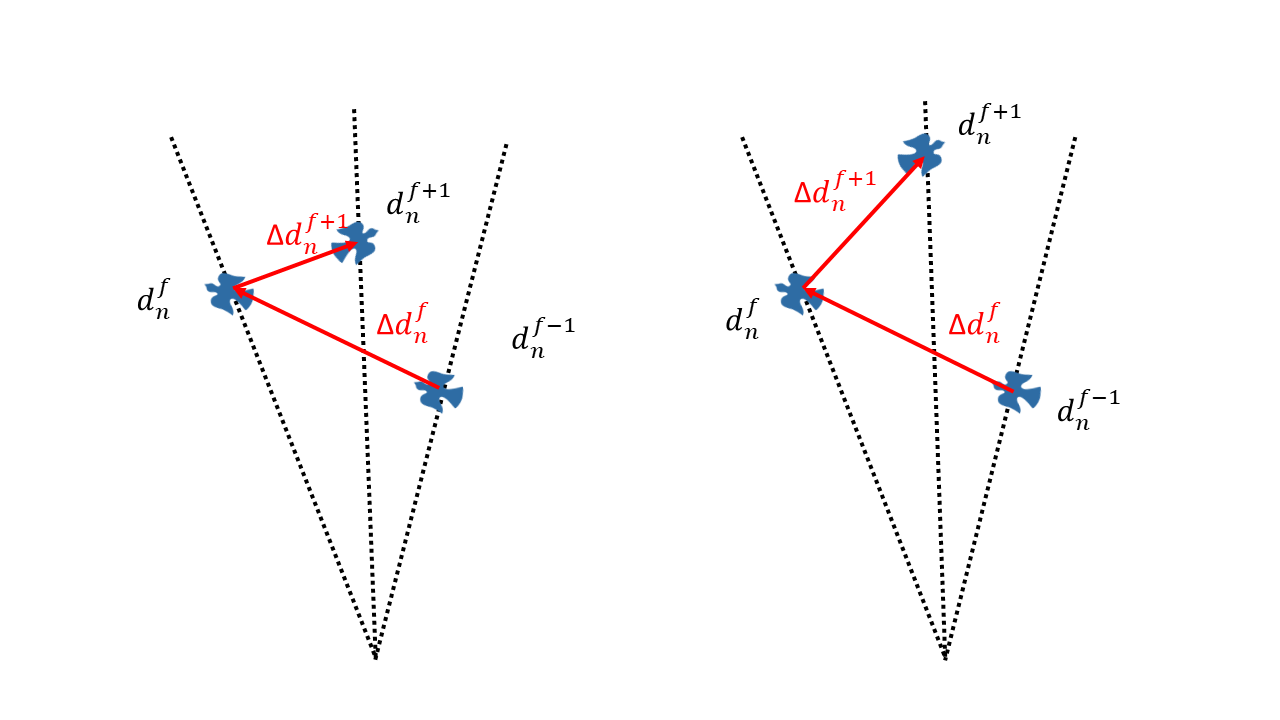
\includegraphics[width=1.0\textwidth]{turn.eps}
 \end{center}
 \caption{Illustration of trajectory smoothness. Figure on the left shows the scenario of sudden turn, while the trajectory on the right is considered a better trajectory, since the speed difference is smaller.}
 \label{figure:turn}
\end{figure}



Trajectory smoothness is the first term in our error function in equation \ref{eq:1}, denoted as $t(.)$. In this term, only the trajectory of one bird is considered. We assume that a bird tends to minimize its velocity change during its flight. The importance of retaining trajectory smoothness is especially obvious when bird is on turning point of the track. In our experiment, we found that if trajectory smooth is not considered, birds will show a sudden turn motion, which is unnatural. Figure \ref{figure:turn} shows the scenario of sudden turn. Trajectory smoothness term is then denoted as:

\begin{equation}\label{eq:4}
 t(p_n^f, p_n^{f-1},d_n^f) = |||v_n^f||-||v_n^{f-1}||| = |||b_n^f-b_n^{f-1}|| - ||b_n^{f-1}-b_n^{f-2}|||
\end{equation}

as first term in error function to be minimized in optimization stage to retain trajectory smoothness.


\section{Flock behavior similarity}


We use Reynolds' boid model as basic flock behaviors. In boid model, each bird in flock, which is called a boid, observes three steering rules: separation, cohesion, and alignment. The definitions of these steering rules rely on the neighbors of the boid. The neighbors of one boid include its surrounding neighbors who are sufficiently close, and each rule has its perceptual neighborhood. Figure \ref{figure:boid} illustrates the definition of three boid rules. As the basic rules of flock behaviors, we believe that more the result matches the boid rules, the better result is. This property is considered as the second term: flock behavior similarity, meaning how close the flock motion shows to flock behavior rules. To calculate flock behavior similarity, target position of boid $n$ in frame $f$ must be calculated first. The target position is then compared with the predicted boid position. Target position is the sum of boid rules. Here we further describe the calculation of the three steering rules.


\begin{figure}[h]
 \begin{center}
  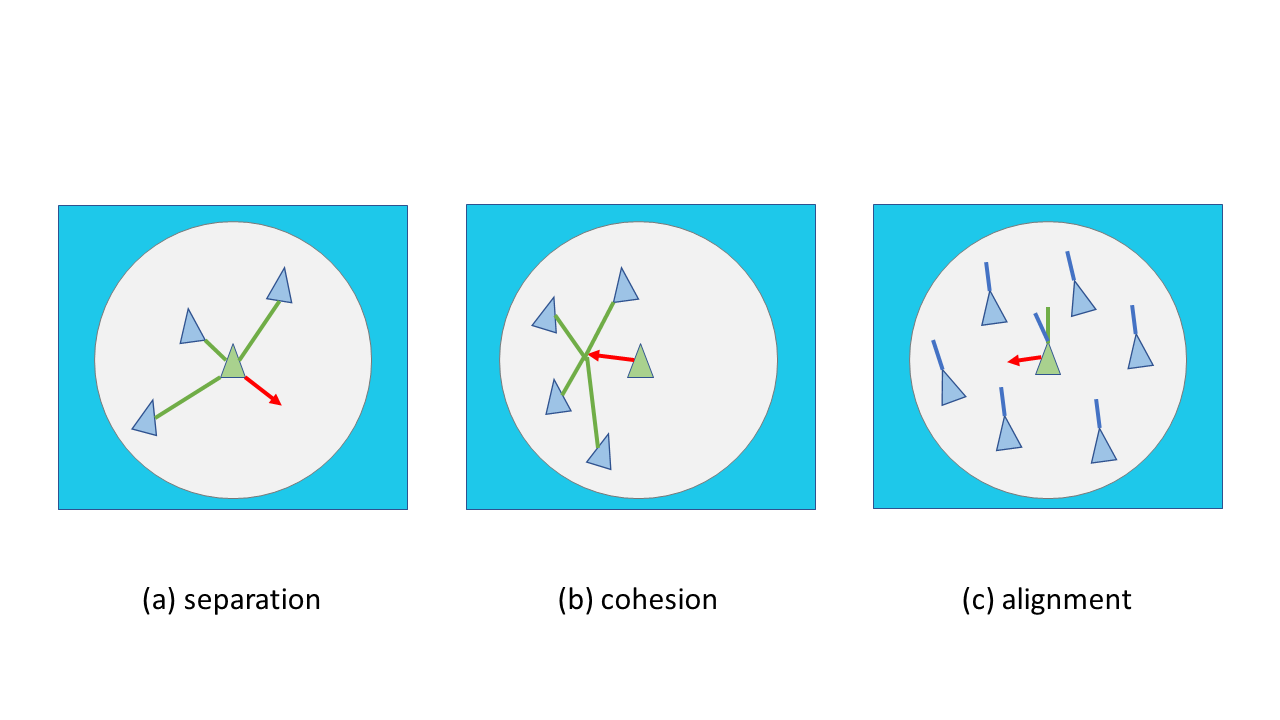
\includegraphics[width=1.0\textwidth]{boid.eps}
 \end{center}
 \caption{Illustration of three boid rules. (a) separation behavior. (b) cohesion behavior. (c) alignment behavior.}
 \label{figure:boid}
\end{figure}


Separation steering behavior, as shown in Figure \ref{figure:boid} (a), gives a boid the ability to maintain a certain separation distance from others nearby and to prevent boids from crowding together. We think that separation rule is the most important rule for creating nature flock motion, since collision with other birds is obviously unnatural. To compute separation force, first a search is made to find other boids within the specified neighborhoods. For each nearby boid, the force is computed by subtracting the positions of the boid and the nearby boids, normalizing, and then applying a $1/r$ weighting, making force of nearer nearby boid stronger. All forces for each nearby boid are summed together to produce the overall separation force.


Cohesion steering behavior, as shown in Figure \ref{figure:boid} (b), gives a boid the ability to approach and form a group with other nearby characters. That is, boids steer towards the average position of the nearby boids. This behavior helps flock to form a group and not be too separated. The neighborhood of cohesion is set much bigger than neighborhood of separation does to keep the flock form in group while preventing collision.


Alignment steering behavior, as shown in Figure \ref{figure:boid} (c), gives a boid the ability to align itself, heading in the same direction with other nearby boids. However, since in the optimization stage, we only consider optimizing position of each boid, we do not use alignment rule here. Instead, we refine the alignment after optimization is done.


\begin{algorithm}[h]
\SetAlgoLined
\tcp{Calculate separation force $\vec{s}$ of bird n}
$\vec{s} \leftarrow \vec{0}$ \;
$neighbor \leftarrow 0 $ \;
\For{$i\leftarrow 1$ \KwTo $N$}{
  \lIf{i=n}{continue}
  $distance \leftarrow ||b_n - b_i||$ \; 
  \If{distance $\leq d_{sep}$}{
    $neighbor \leftarrow neighbor+1$ \;
    $\vec{s} \leftarrow \vec{s} + (b_n - b_i) / distance$ \;
  }
}
$\vec{s} \leftarrow \vec{s} / neighbor$ \;
\caption{Calculation of separation vector $\vec{s}$}
\label{algo:separation}
\end{algorithm}


\begin{algorithm}[h]
\SetAlgoLined
\tcp{Calculate cohesion force $\vec{c}$ of bird n}
$\vec{c} \leftarrow \vec{0}$ \;
\For{$i\leftarrow 1$ \KwTo $N$}{
  \lIf{i=n}{continue}
  $\vec{c} \leftarrow \vec{c} + (b_i - b_n)$ \;
}
$\vec{c} \leftarrow \vec{s} / (n-1)$ \;
\caption{Calculation of cohesion vector $\vec{c}$}
\label{algo:coherence}
\end{algorithm}


Combining rules above, now we can calculate flock behavior similarity term $f(.)$ in equation \ref{eq:2} by calculating Euclidean distance between the target position and predicted position. Algorithms of calculating separation and cohesion are shown in Algorithm \ref{algo:separation} and \ref{algo:coherence}. In calculating separation vector $\vec{s}$, a neighborhood distance $d_{sep}$ is set to decide the minimum distance to keep in flock motion between each birds. Tuning this parameter, which can be done by user in optimization stage, is considered as an interactive element in our system. In boid algorithm, a neighborhood of cohesion is also set. However, since we assume all birds in input video belong to one flock that are aware of each other, we just consider every birds in the flock for calculating cohesion force. This can also reduce number of parameters while keeping other parameters more focused.


In most flock simulation approaches, collision is detected in advance by adjusting its direction and speed when other agents are about to collide. In our flock model, since we have separation rule that separate, birds tend to move away to each other when they are too close. Therefore, we do not handle collision avoidance.


\section{Frame-by-frame optimization}

\begin{algorithm}[h]
\SetAlgoLined
\KwData{Trace set $X=\big\{d_n^f\big\}$}
%\KwResult{how to write algorithm with \LaTeX2e }
\tcp{Algorithm start}
Scatter bird positions in frame 1 \;
\tcp{Frame-by-frame optimization}
\For{$i\leftarrow 2$ \KwTo $F$}{
  $sum \leftarrow 0$ \;
  \For{$j\leftarrow 1$ \KwTo $N$}{
    $\vec{v} \leftarrow b_j^i - b_j^{i-1}$ \;
    \If{i = 2}{
      \tcp{Initial speed}
      $sum\leftarrow sum + || ||\vec{v}|| - v_{target}||$ \;
    }
    \Else{
      \tcp{Trajectory smoothness}
      $\vec{v_{last}} \leftarrow b_j^{i-1} - b_j^{i-2}$ \;
      $sum\leftarrow sum + \lambda_{t}|| ||\vec{v}|| - ||\vec{v_{last}}||  ||$ \;      
      \tcp{Flock behavior similarity}
      Calculate separation force $\vec{s}$ \;
      Calculate cohesion force $\vec{c}$ \;
      $target \leftarrow b_j^{i-1} + (w_{sep} \vec{s}+(1-w_{sep})\vec{c})$ \;   
      $sum\leftarrow sum + \lambda_{f}|| b_j^i - target  ||$ \; 
    }
  }
  Minimize $sum$ \;
}

\caption{Optimization algorithm.}
\label{algo:optimization}
\end{algorithm}



The task in our optimization stage is to minimize error function equation \ref{eq:1} with target depth set $X$. Totally, since we have track data of $N$ birds in $F$ frames, there are $N{\times}F$ target depths. If the optimization is done globally, the computation time will be costly. Since our goal is to make system that user can adjust the result interactively in real time, we consider doing the optimization frame-by-frame. Frame-by-frame optimizations means we do not optimize Equation \ref{eq:1} directly, instead, we predict $N$ depths in frame $f$ from the first frame to next frame, based on the results from last frames. That is, to optimize Equation \ref{eq:2} for $n=1...N$ This approach greatly decreases computation time, making it possible for user to do the optimization and see the result interactively while adjusting parameters.


To prevent optimization result make bird flock fly too far or too near to the camera, as inequality constraints in optimization algorithm, a near and a far constraint of depth are set as:


\begin{equation}\label{eq:depth}
d_{near} < d < d_{far}
\end{equation}


However, since constraints $d_{near}$ and $d_{far}$ does not affect the result much. It only avoid flock fly too near or too far to the camera, which seldom happens. Therefore, we do not consider these two parameters as interactive elements for user. Since target error function can be calculated in each frame, with the inequality constraint \ref{eq:depth}, after optimization is done in every frame, optimized $X$ can be found as result.


Algorithm \ref{algo:optimization}  shows our optimization algorithm. As mentioned above, our frame-by-frame optimization optimizes each frame based on the result from last frames. However, we do not have any previous frame for the first frame. Therefore, we have to decide the initial positions of $N$ birds in the first frame. This part can also be discussed in many aspects. However, we decide to make this part simple: just scatter it in the range within $d_{near}$ and $d_{far}$ randomly, with at least a distance between them.


After the positions of birds in the first frame are decided, next is the second frame. Since the distance of bird positions between frame 1 and frame 2 greatly affects optimization in later frames, the position in frame 2 is important. Here, we use a user-defined speed factor $v_{target}$ as a reference to decide the positions in frame 2. We simply spawn birds in frame 2 in position that approximate the defined distance $v_{target}$ to the position in frame 1.


The reason why we do not dig in the part of deciding initial positions is that it is less important than how trajectory shows in flock motion, since our goal is not to reproduce the original flock motion. That is, how initial positions are decided does not affect the evaluation of the result. Thus, we focus on the transition of bird flock rather than initial position. 


After the positions in frame 1 and 2 are decided, now we can apply the rule of trajectory smoothness and flock behavior similarity based on positions in previous frames. The first term, trajectory smoothness, is calculated as velocity difference between this frame and last frame. The second term, flock behavior similarity, is calculated as sum of separation force $\vec{s}$ and cohesion force $\vec{c}$, which are shown in \ref{algo:separation} and \ref{algo:coherence}. We balance these two force using parameter $w_{sep}$, which is considered as an interactive element in our system. As mentioned in section 3.4, separation force prevents birds from colliding, while cohesion force keeps flock stay together. Final force is decided as $(w_{sep} \vec{s}+(1-w_{sep})\vec{c})$. By tuning $w_{sep}$ from 0 to 1, the user can decide the flock in result to scatter or gather. After two terms are decided, we also balance the two terms are by two parameters: $\lambda_{t}$ and $\lambda_{f}$, balancing the trajectory smoothness and flock simulation similarity. After the sum of two terms are calculated, it is optimized by changing $d_n^f$. After the optimal depth $d_n^f$ is solved by the optimization algorithm, the system moves to next frame until all frames are done.


We implement the optimization part using NLopt library \cite{NLopt} with optimization algorithm constrained optimization by linear approximation (COBYLA)\cite{COBYLA}.



\section{Modeling flock motion}


After we get the optimized depth data, next step is to visualize the optimized flock motion. We implement the visualization with Unity\cite{Unity}. And optimization system is loaded as plugin to make it can be used in an interactive way.


In optimization stage, the position of each bird in every frame is predicted. However, since the system only finds optimal position of each bird, orientation needs to be assigned to complete flock motion. Here we just simply decide orientation of each bird frame-by-frame based on its current position and position in last frame. First, the orientation vector of bird $n$ in frame 2 is simply decided by position difference $\vec{o}_n^f=d_n^2 - d_n^1$. After that, we just interpolate position difference vector and previous orientation $\vec{o}$ with parameter $0.1$ in every frame, meaning that the orientation is slightly changed each frame while keeping its previous orientation. We use interpolation here because sometimes the result seem weird because of errors in original track data, causing birds changing orientation frequently.


\section{Interactive user interface}


\begin{figure}[h]
 \begin{center}
  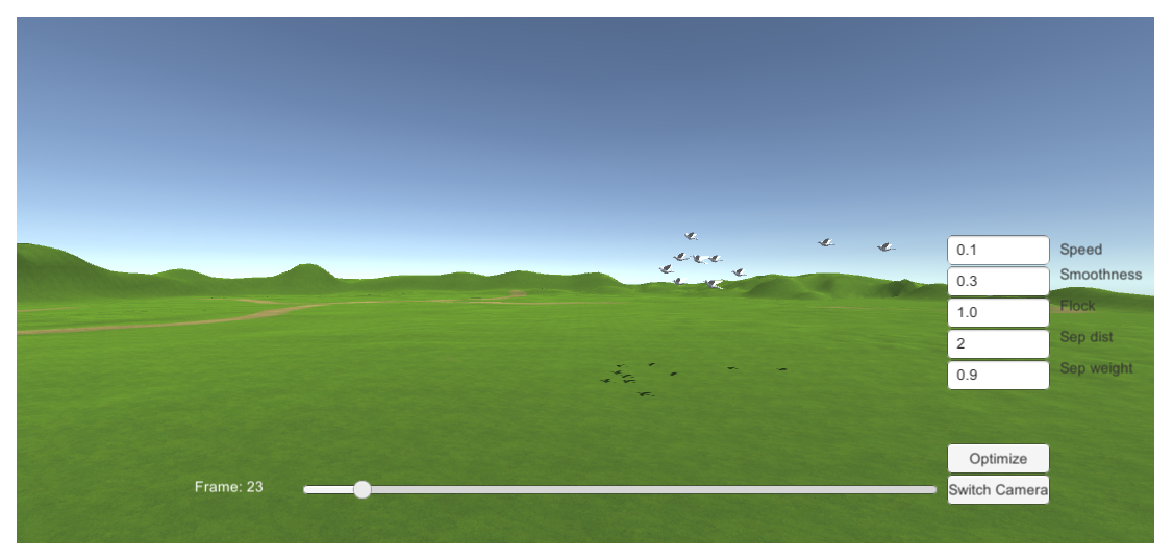
\includegraphics[width=1.0\textwidth]{ui.eps}
 \end{center}
 \caption{User interface of our system in optimization stage.}
 \label{figure:ui}
\end{figure}


By now, we have introduced 5 parameters for optimization stage: $v_{target}$ for target speed of each bird, $\lambda_{t}$ for weight of trajectory smoothness, $\lambda_{f}$ for weight of flock behavior similarity, $d_{sep}$ for neighborhood distance for separation rule, and$w_{sep}$ for weight of separation rule. In our system, these parameters are treated as interactive elements of our system. Since the optimization can be done in seconds, user can see the result and adjust parameter can do the optimization again to get better results. Figure \ref{figure:ui} illustrates our user interface. With our interactive user interface, user can move camera to check the result in each frame. 5 parameters can be edited by the text fields on the right part of the screen, and the slider on the bottom part of the screen can adjust the frame shown. User can also switch between top-view camera and side-view camera by pressing switch button.